\chapter{Engineering Thermal Processes in Semiconductor Nanocrystals}

Work in this Chapter is adapted from the following papers:
\begin{itemize}
\item Hannah, D.C.; Ithurria, S.; Krylova, G.; Talapin, D.V.; Schatz, G.C.; Schaller, R.D. \emph{Nano Letters} \textbf{2012} 12, 5797
\end{itemize}

Theoretical work in this Chapter is adapted, in part, from the following papers:

\begin{itemize}
\item Rowland, C.E.; Liu, W.; Hannah, D.C.; Chan, M.K.Y.; Talapin, D.V.; Schaller, R.D. \emph{ACS Nano} \textbf{2013}, 8, 977
\item Rowland, C.E.; Hannah, D.C.; Demortiere, A.; Yang, J.; Cook, R.E.; Prakapenka, V.B.; Kortshagen, U.R.; Schaller, R.D. \emph{ACS Nano} \textbf{2014}, 8, 9219
\end{itemize}

\section{Overview}

While much research involving NCs examines optical and electrical processes such as charge separation and transport, phonon transport is equally critical to many device applications. Specifically, thermoelectrics benefit from minimal phonon transport as power conversion efficiency relates inversely to thermal conductivity \cite{doi:10.1021/cm902195j} whereas optical sources such as LEDs and lasers \cite{doi:10.1021/nl9002969,Klimov13102000} require maximal transport where high thermal conductivity improves brightness at high currents and extends operational longevity \cite{Narendran2004449}.  Spatially periodic arrays of scattering centers have been demonstrated as a top-down means to manipulate phonon transport \cite{cheng2006observation,PhysRevLett.94.115501,doi:10.1021/nl102918q,PhysRevLett.100.194301}, but this scheme presents inherent problems for many applications since it necessitates higher-order material organization. Rather, component-level, bottom-up engineering of phonon transport via direct tuning of the NC thermal properties imposes fewer requirements on the overall structure, which in some cases may comprise only a single active NC layer \cite{doi:10.1021/nl9002969}. Ideally, for a given application, one would like to separately select the semiconductor component energy gap as well as the material thermal conductivity for optimal device operation. \par

In this Chapter, we demonstrate using a combination of experimental characterization and theoretical modeling that appropriate modification of semiconductor nanocrystal surfaces can manipulate thermal transport rates independently of optical properties and improve the thermal stability of semiconductor NC materials at the single particle level.

\section{Particle-Level Engineering of Thermal Conductivity in Matrix-Embedded Semiconductor Nanocrystals}

As detailed in Chapter 3, non-contact characterization of thermal transport from NCs has been achieved by monitoring optical signatures of phonon outflow arising from transient phonon-assisted radiative recombination from the lowest-energy exciton fine structure state (the “dark” exciton state), for which transitions are ordinarily dipole-forbidden. As schematically described in Figure \ref{f:plevel1}(a) for a NC initially at a very low temperature (3 K), ultrafast intraband relaxation of excited charge carriers produces dark-excitons and nonequilibrium phonons typically within $\sim$1 ps following excitation. Acoustic phonons in particular impart distortions of the NCs that transiently perturb exciton fine structure and assist in angular momentum conserving radiative transitions \cite{:/content/aip/journal/jcp/132/10/10.1063/1.3350871,doi:10.1021/jp201408m}. As a result, rapid phonon-mediated radiative recombination occurs with a higher photon generation rate during the period of time in which the NC contains acoustic phonons, than in unperturbed NCs containing a dark exciton (Figure \ref{f:plevel1}(b)).  As time progresses, these phonons flow out from NCs into the surrounding matrix on a time scale consistent with diffusion-limited thermal transport. Following the outflow of acoustic phonons, radiative recombination occurs via concurrent emission of a photon and a 25-meV longitudinal optical (LO) phonon, which gives rise to a NC-size independent spectral red-shift between early- and late-time emission spectra (Figure \ref{f:plevel1}(c)). Despite the early-to-late PL energy shift, spectral linewidths over this time range remain constant, consistent with a single population evolving in time to emit at a lower energy. The slower radiative rate of the late-time LO-phonon-assisted recombination process results in fewer detected photons per unit time subsequent to the outflow of acoustic phonons. The initial spike in emission intensity is only apparent at low temperatures (though we expect the physics presented is relevant for higher temperatures), since at high sample temperatures (near 80 K) an equilibrium population of acoustic phonons in NCs exists that does not decay to zero with time. That is, the perturbation from acoustic phonons persists continuously at higher temperatures \cite{PhysRevLett.107.177403}.

\begin{figure}
\begin{center}
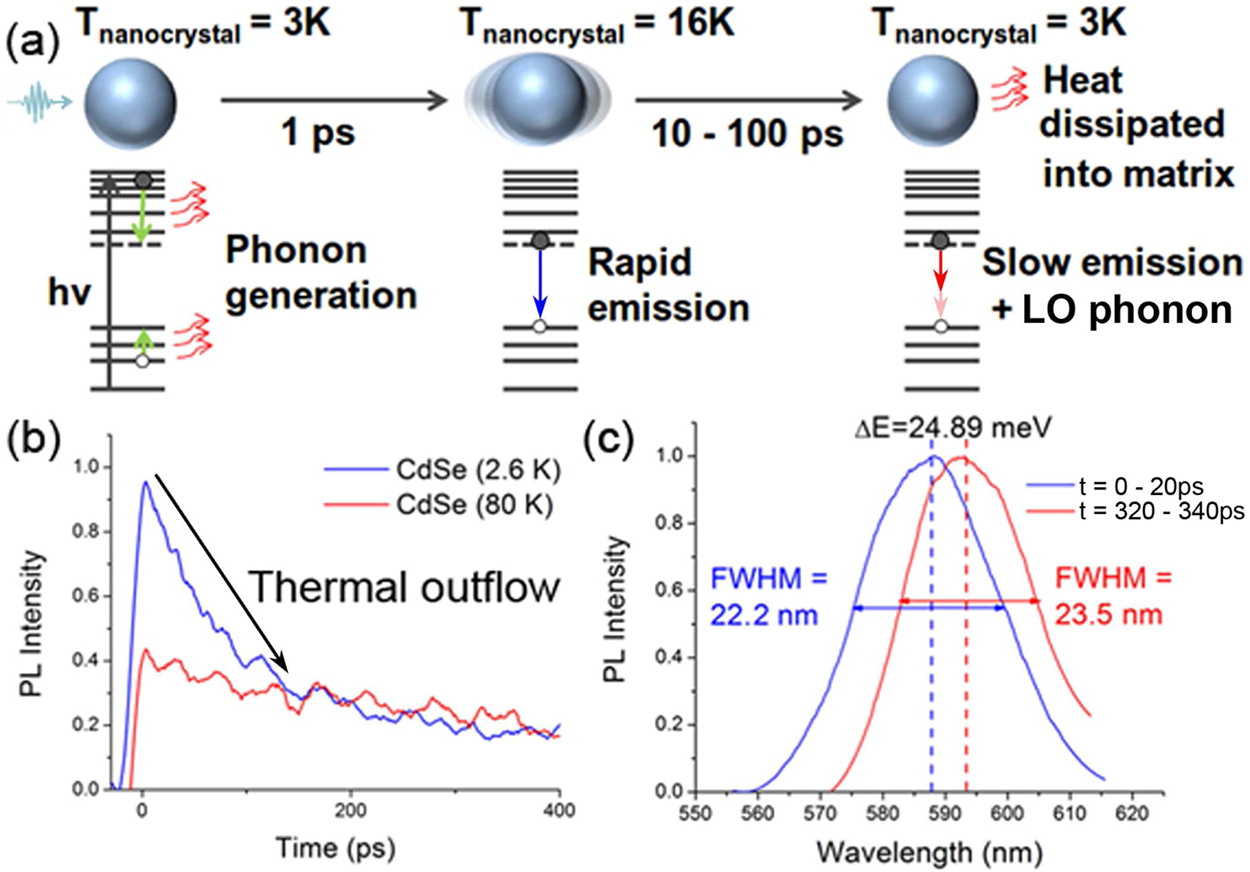
\includegraphics[width=0.75\textwidth]{./Chapter5/plevel1.jpeg}
\caption[Synopsis of thermal outflow detection in CdSe NCs.]{Synopsis of thermal outflow detection in CdSe NCs. (a) A photoexcited NC at low temperature (3 K) undergoes intraband relaxation on a $\sim$1 ps time scale, resulting in the population of lattice vibrations and dark excitons. Subsequent to thermalization with the surrounding matrix, radiative recombination of dark excitons occurs via a LO-phonon assisted mechanism, resulting in microsecond radiative lifetimes. (b) Dynamics for a 3.8-nm diameter CdSe NC are shown at 3 and 80 K; biexponential dynamics are observed at 3 K. The rapid emission feature corresponding to thermal outflow from NCs is indicated. (c) Representative time-resolved emission spectra for matrix-embedded CdSe NCs at 3 K. The 25-meV red-shift with increasing time is consistent with initial acoustic phonon assisted PL followed by 25-meV LO-phonon assisted PL, while the consistent line width (indicated) suggests a single population evolves in time.}
\label{f:plevel1}
\end{center}
\end{figure}

Here, using the above-described transient PL (trPL) technique, we report measurements of heat transport time scales for matrix-embedded semiconductor NCs with the goal of manipulating thermal outflow times. Upon growing an electronically noninteracting ZnS shell of controlled thickness, we show that the phonon outflow time increases significantly. In particular, we find that the fitted lifetime of the exponential decay related to phonon transport increases with increasing ZnS shell thickness for a fixed CdSe NC core size. We also measure numerous core-shell samples comprising different core sizes and determine that the phonon outflow time follows the overall particle size. These findings shows that phonon outflow times can be tuned separately from the optical energy gap via manipulation of the overall particle size at the component level. \par

Near-spherically shaped CdSe NCs were synthesized using a previously described seeded-growth approach \cite{doi:10.1021/nl0717661}.  ZnS shell-growth also followed a previously described procedure, summarized here \cite{doi:10.1021/nl0155126}. A solution of as-synthesized CdSe NCs was heated and mixed with trioctylphosphine oxide and hexadecylamine. A Zn:S stock solution was added dropwise to the CdSe NC solution and stirred vigorously. The amount of stock solution necessary to obtain a desired shell thickness was calculated from the ratio between core and shell volumes using bulk lattice parameters of CdSe and ZnS. Samples were characterized by optical absorption and emission as well as transmission electron microscopy (TEM). For optical experiments, NCs were dissolved in molten octadecane and drop cast onto a sapphire disk. The volume fraction of NCs was <1\% for all presented experiments. Samples were loaded into a closed-cycle helium cryostat and excited with 35-fs pump pulses at 2 kHz with 3-eV photon energy. To ensure single-exciton dynamics, pump fluence was adjusted such that the average number of excitons per NC was less than 1. Four times higher or lower fluence did not alter observed dynamics (see Appendix A). \par

\begin{figure}
\begin{center}
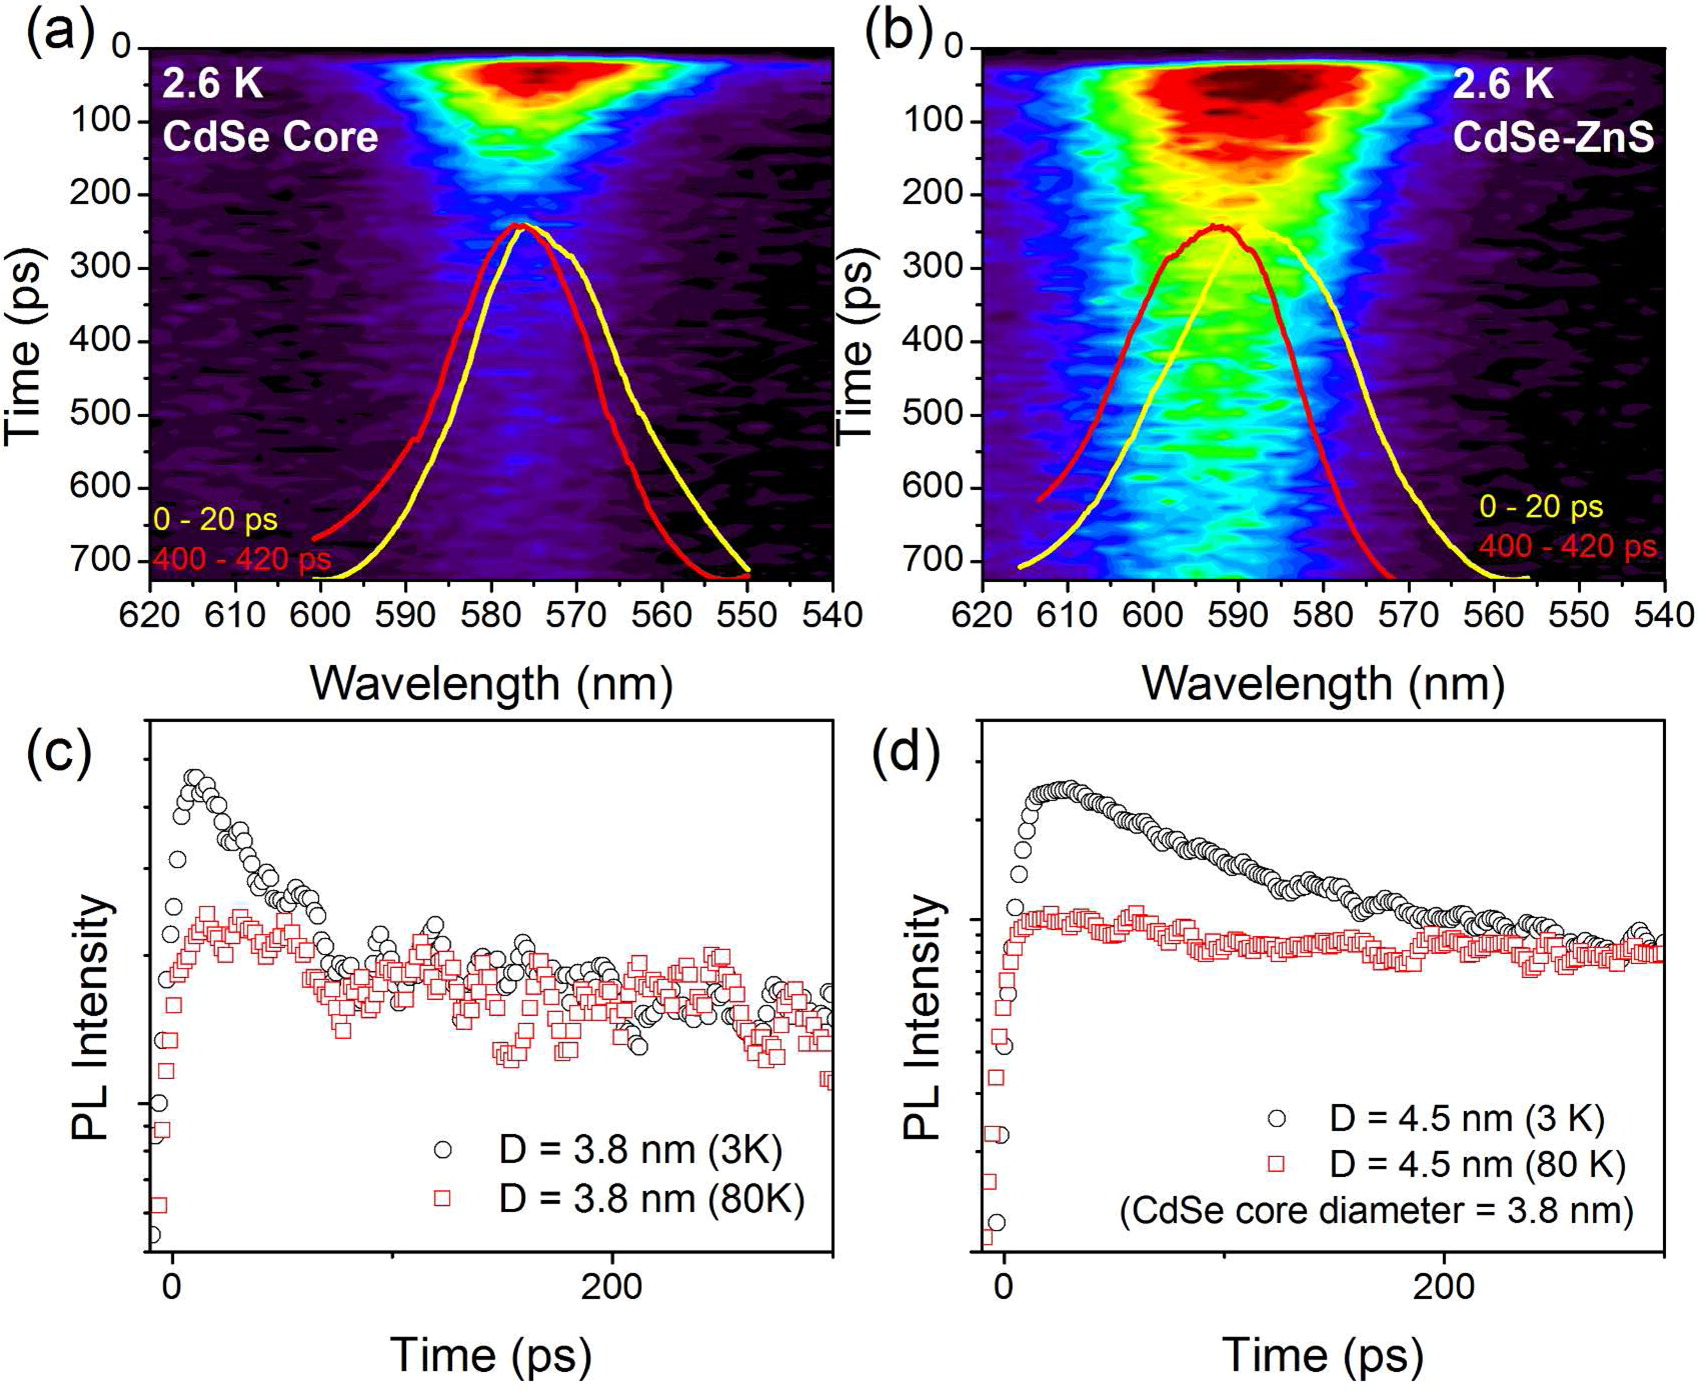
\includegraphics[width=0.75\textwidth]{./Chapter5/plevel2.jpeg}
\caption[Comparison of PL decay dynamics between core-only and core-shell CdSe NCs.]{(a) A streak camera image for a 3.8-nm diameter core-only CdSe NC photoexcited at 3 eV. The spectral overlays show time-integrated emission from $t = 0 - 20$ ps (yellow) and $t = 400 - 420 ps$ (red). (b) The same for a 4.5-nm diameter CdSe-ZnS core-shell NC with the same 3.8-nm diameter CdSe core as in panel a. (c) Comparison of PL dynamics at 2.6 K (black circles) and 80 K (red squares) for the 3.8-nm CdSe core-only sample and (d) for the 4.5-nm CdSe-ZnS core-shell sample. Note the longer time scale of the low-temperature decay feature in d.}
\label{f:plevel2}
\end{center}
\end{figure}

Figure \ref{f:plevel2}(a) and (b) shows subnanosecond streak-camera images of trPL recorded at 2.6 K for a 3.8-nm diameter ($D$) CdSe NC core (Figure \ref{f:plevel2}(a) and the same core size overcoated with a wide-gap ZnS shell to yield a 4.5-nm CdSe-ZnS core-shell particle (Figure \ref{f:plevel2}(b)). We display time-resolved spectra integrated for $t = 0-20$ ps (early) and $t = 400-420$ ps (late) superimposed on the streak camera images. A clear 25-meV red-shift from early to late time, which appears for all samples examined, matches the LO-phonon energy of bulk CdSe (see above). Figure \ref{f:plevel2}(c) and d shows dynamics for both a core-only and a core-shell NC sample that have been spectrally binned for wavelengths to the blue of the late-time PL band center (“blue-side” dynamics), which emphasizes the fast decay component. Both samples clearly exhibit an initial subnanosecond decay component at 2.6 K that is not observed at 80 K (as shown in Figure \ref{f:plevel2}(c) and (d)). Notably the fast feature decay lifetime becomes significantly longer for the core-shell sample. The elevation of the sample temperature to 80 K causes a loss of the fast feature amplitude relative to the late-time amplitude, which we previously showed for CdSe core-only NCs was consistent with Boltzmann thermal partitioning \cite{PhysRevLett.107.177403} with acoustic phonon energies spanning 0.8-1.8 meV. As rapid emission appears acoustic-phonon mediated, the difference in lifetime between the core and the core-shell samples (Figure \ref{f:plevel2}(c) and (d)) suggests that acoustic phonon dissipation times might be controlled via the overall particle size. \par

To begin with, the elastic constants of CdSe and ZnS are similar ($\rho_{CdSe} = 5816$ g/m$^3$, $\rho_{ZnS} = 4075$ g/m$^3$, $v_{sound, CdSe} = 3559$ m/s, $v_{sound, ZnS} = 3868$ m/s), which suggests a small acoustic impendence mismatch at the CdSe-ZnS interface, in comparison to the semiconductor-to-organic interface. Grossly approximating as a planar interface, calculations based on the acoustic mismatch model for the CdSe-to-ZnS interface yield a phonon transmission coefficient of 0.99, whereas the ZnS-to-organic interface yields nearly an order of magnitude lower value of only 0.15. As a result, heat deposited in the CdSe core due to intraband relaxation likely distributes rapidly throughout the entire core-shell structure. Previously we showed that thermalization of a NC lattice with its environment closely followed diffusion-limited times for thermal outflow \cite{PhysRevLett.107.177403}. Diffusion-limited thermal outflow time depends proportionately on the surface area of the NC in contact with the matrix. Therefore, we attempted to modify particle thermalization rates for CdSe-ZnS core-shell NCs by manipulating the overall particle size. \par  

Figure \ref{f:plevel3} relates the dependence of total particle size on thermal outflow time. Here, we subtract the slow emission component observed at long times from early PL amplitude to emphasize the early time exponentially decaying component. Figure \ref{f:plevel3}(a) depicts PL dynamics for a series of CdSe core-only samples of increasing size. Lifetimes increase for larger CdSe NC radii, where the smallest sample exhibits a thermal outflow lifetime of 10.3 ps and the largest core-only sample presents a lifetime of 106.7 ps. Figure \ref{f:plevel3}(b) presents data for samples wherein overall particle size increases via the growth of a progressively thicker ZnS shell on a fixed-size CdSe core. For this fixed, intermediate-sized CdSe core, the rapid-emission lifetime increases from 25.9 ps in the smallest core-shell NC to 130.3 ps in the largest core-shell NC. The relationship between overall particle size (including core and shell) and thermal outflow lifetime for various CdSe core-only NCs and random shell-thickness CdSe-ZnS NCs is plotted in Figure \ref{f:plevel3}(c). This comparison illustrates that overall particle size heavily dictates phonon outflow time. Figure \ref{f:plevel3}(d) displays thermal outflow times for a series CdSe cores of increasing size as well as for a series of fixed-size CdSe cores with a ZnS shell of increasing thickness. From this comparison, it is apparent that thermal outflow time can be tuned largely independently of the emission energy, which is dictated by the core size. Specifically, in the case of core-only samples, emission energies ranging from blue-green (2.6 eV) to red (1.9 eV), a shift of 700 meV, yield thermal outflow times that differ by roughly a factor of 9. On the other hand, thermal outflow times from the smallest to largest CdSe-ZnS (with a fixed core size) sample differ by a factor of 5 with a commensurate emission energy shift of only 90 meV. Thus, shell thickness manipulation demonstrates two points. First, shell thickness manipulation can separate the nominal codependence of the energy gap from thermal outflow time. Second, the demonstrated manipulation of the fast decay dynamics using a nonelectronically interacting shell further supports the notion that the observed dynamics are extrinsic in relation to properties of the core. \par

\begin{figure}
\begin{center}
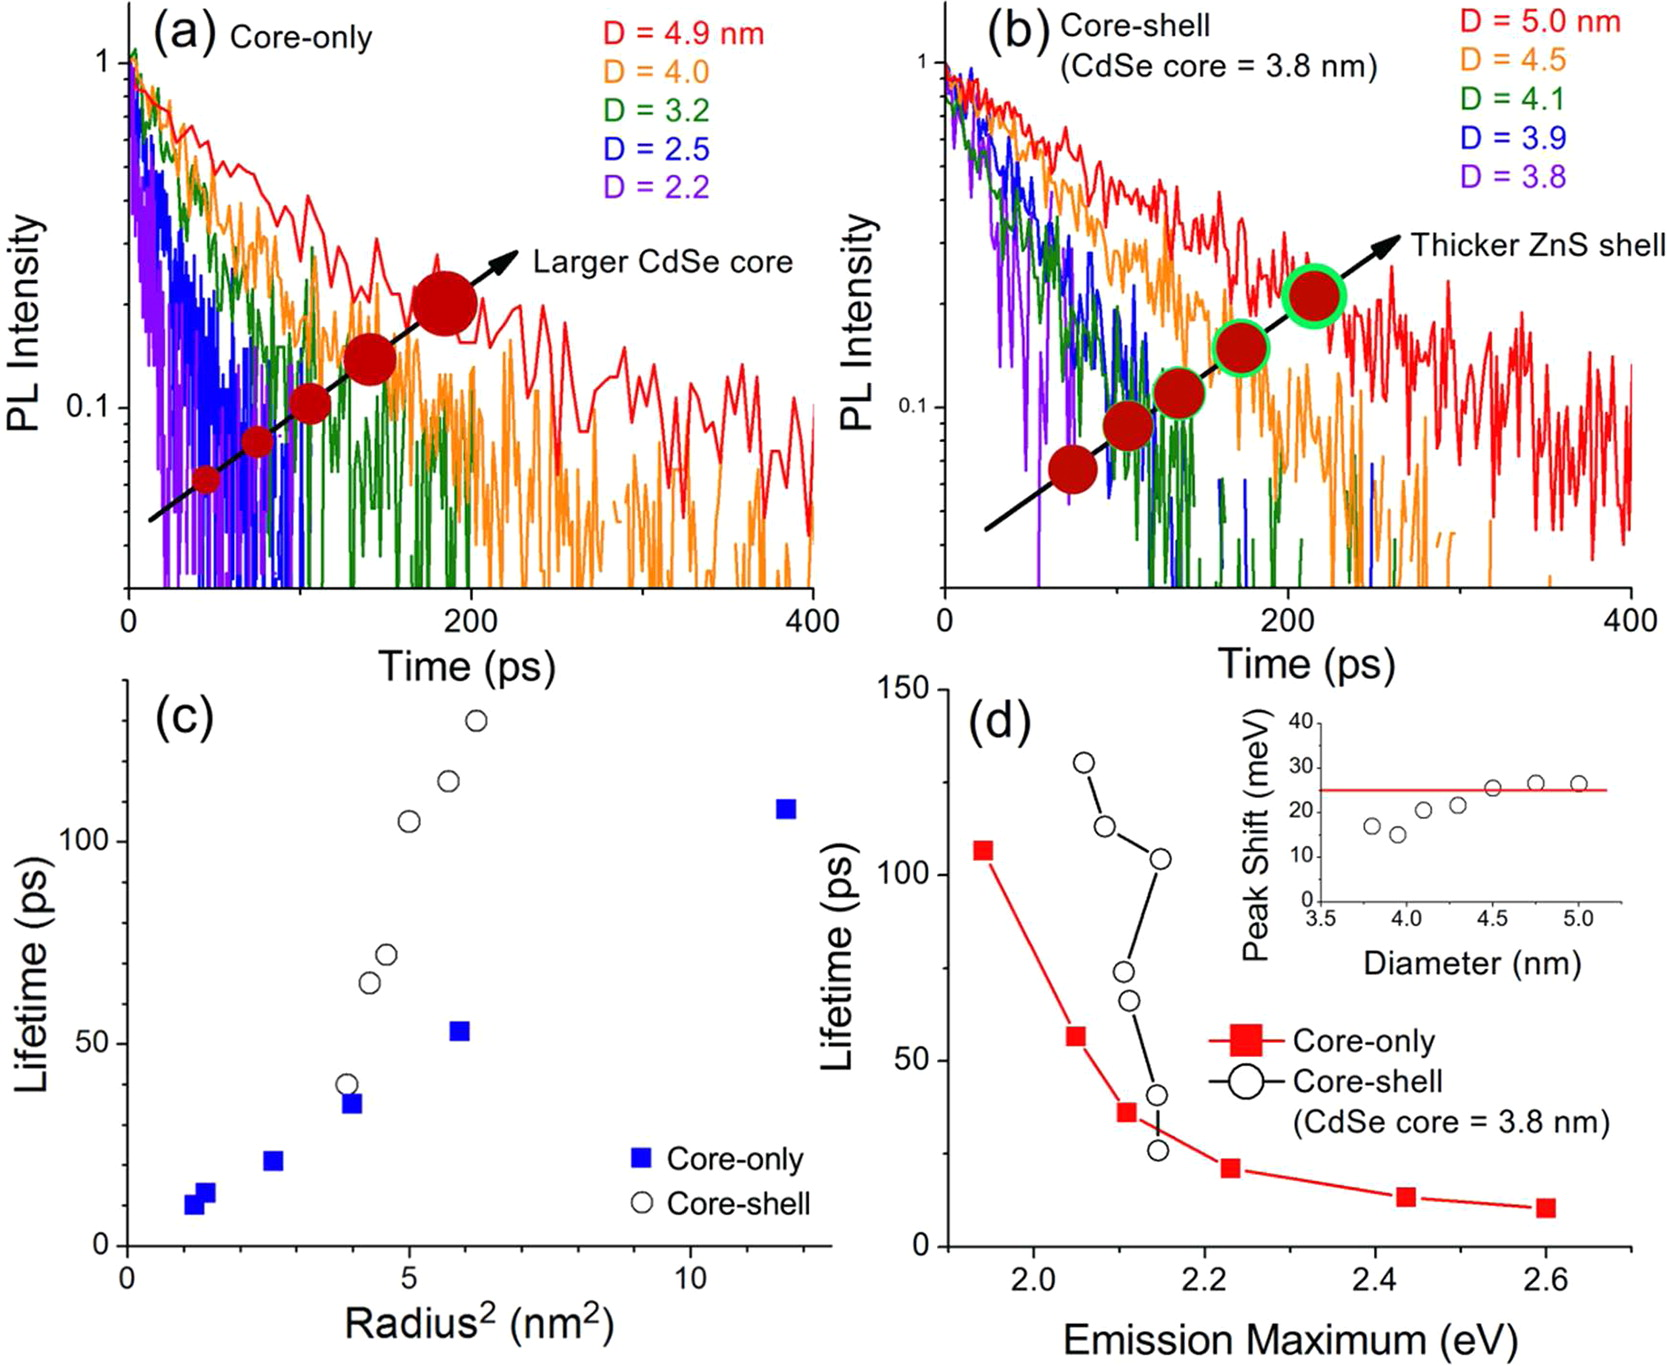
\includegraphics[width=0.75\textwidth]{./Chapter5/plevel3.jpeg}
\caption[PL decay dynamics as a function of particle size and emission energy for core-only and core-shell CdSe NCs.]{(a) Radiative recombination dynamics at 2.6 K produced by spectrally integrating the higher-energy half, or “blue-side”, of the time-integrated PL spectrum for CdSe core-only NCs with indicated diameters. Here, the late-time amplitude has been subtracted from all PL traces to emphasize the subnanosecond decay dynamics. All data have been normalized at early time. (b) Blue-side radiative recombination dynamics for a set of CdSe-ZnS core-shell NCs. For each diameter indicated, the core-shell structure contains a fixed-size 3.8-nm diameter CdSe, while the diameter indicated represents the overall particle size. (c) The blue-side fast-feature decay lifetime measured at 2.6 K for CdSe core-only NCs (blue squares) and CdSe-ZnS core-shell NCs (open black circles) as a function of the radius squared. Note that the x-axis does not convey emission energy because ZnS shells only weakly affect CdSe core emission. (d) Lifetimes of the rapid emission feature as a function measured PL energy at 2.6 K. Emission energy was determined as the maximum of the time-integrated PL data. The red squares indicate CdSe core-only samples, while the open black circles represent CdSe-ZnS core-shell NCs with a 3.8-nm fixed core-size. Inset: Energy shift from early time PL ($t = 0 - 20$ ps) vs late-time PL ($t = 400 - 420$ ps) for the core-shell NCs with indicated fixed-core diameter and varied thickness ZnS shell.}
\label{f:plevel3}
\end{center}
\end{figure}

By modifying the time scale of thermal outflow from the NCs, the growth of an increasingly thick ZnS shell changes the effective thermal conductivity of the composite material constituted by the NCs embedded in an alkane matrix. We estimate the effective thermal conductivity of this system according to Fourier’s law (for spherical particles), yielding the expression $k_{\mathrm{eff}} = \Delta Q/(4\pi R_{NC}\Delta t\Delta T)$.  In this scenario, $\Delta Q$ is the difference in energy between the excitation source and the NC energy gap; it reflects the amount of energy deposited into the NC lattice during intraband carrier cooling and dispersed as heat (Figure \ref{f:plevel1}(a)).  Here, $R_{NC}$, the NC radius, includes the ZnS shell thickness. Acoustic phonon thermal outflow time, as characterized by the lifetime of the rapid emission feature described above, which we point out may be sensitive to the departure time of the last acoustic phonon in the particle, gives $\Delta t$. Finally, $\Delta T$ is given by the difference in temperature between the hot NC lattice and the surrounding matrix. In Figure \ref{f:plevel4}, the effective thermal conductivity ($k_{\mathrm{eff}}$) for a series of matrix-embedded CdSe core-shell NCs decreases with increasing particle size. Increasing the thickness of a ZnS shell thus modifies $k_{\mathrm{eff}}$ of the system from 0.01 W/m/K to 0.002 W/m/K in a controlled manner without modifying the electronic structure of the NCs.  We estimate that for temperatures near 300 K, these $k_{\mathrm{eff}}$ values increase by a factor of $\sim$5 overall, but retain the same functional form.

\begin{figure}
\begin{center}
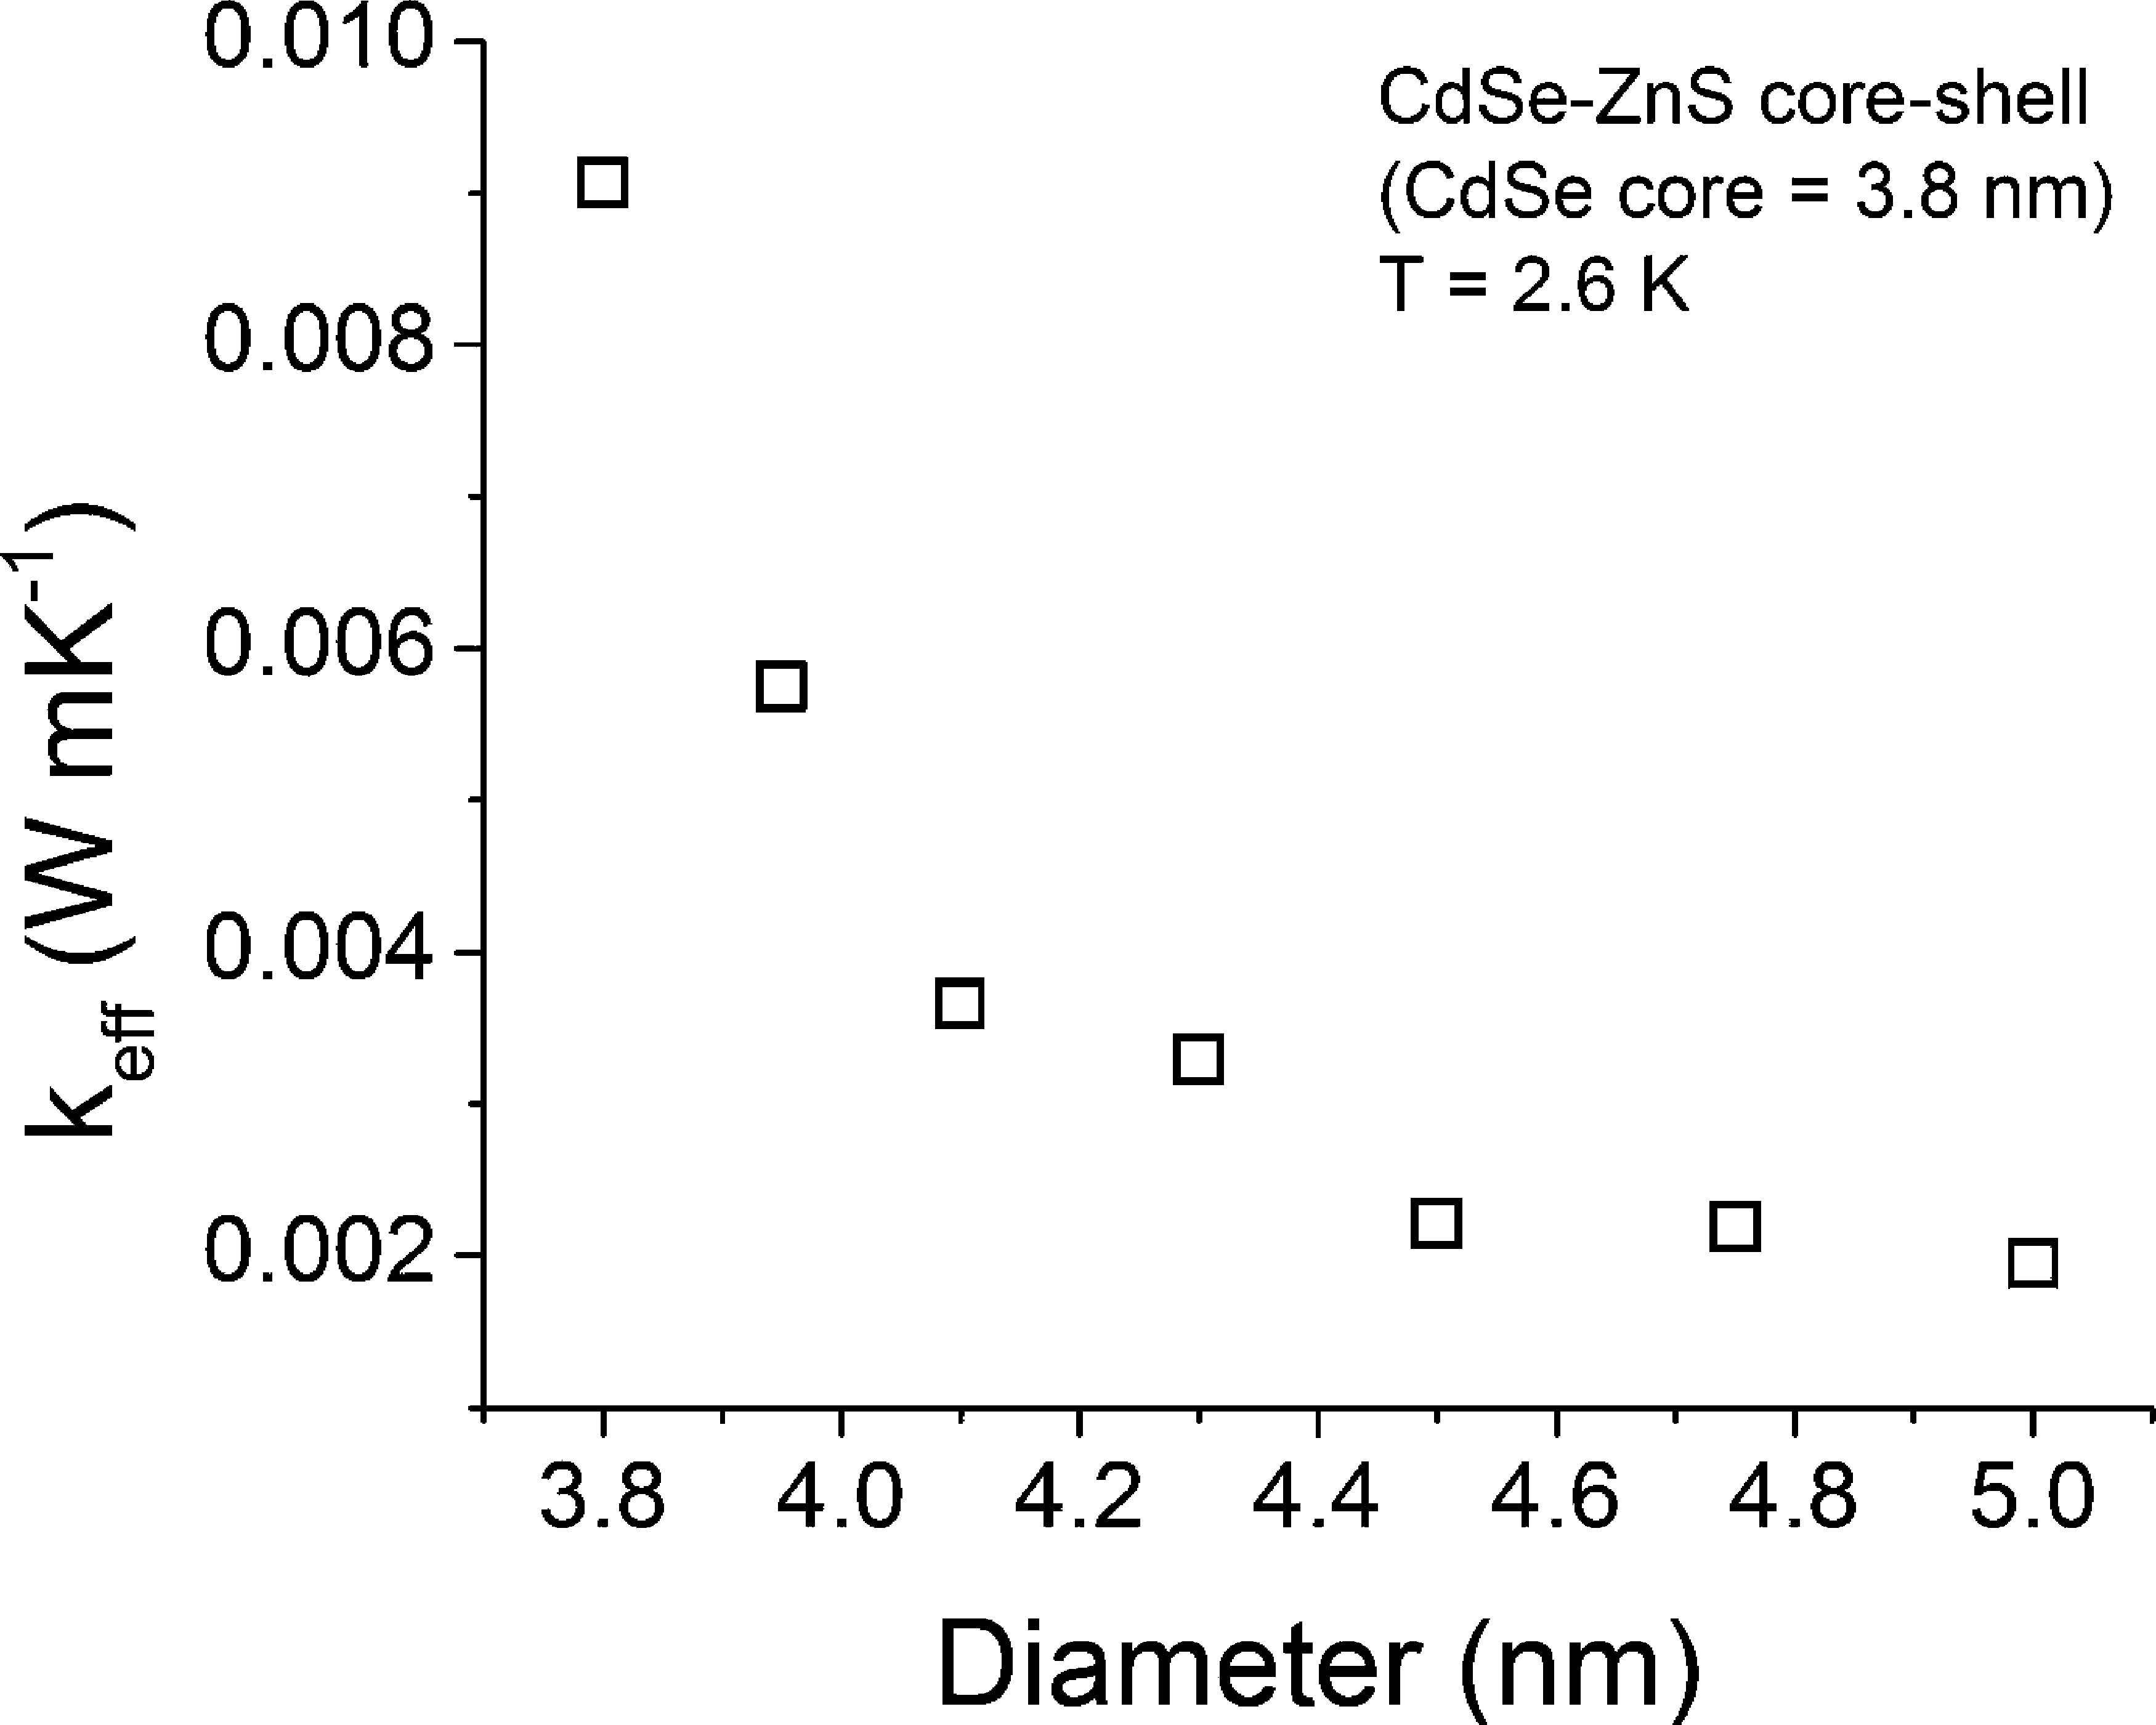
\includegraphics[width=0.75\textwidth]{./Chapter5/plevel4.jpeg}
\caption[Low-temperature effective thermal conductivity as a function of NC diameter for a series of CdSe-ZnS core-shell NCs embedded in an octadecane matrix.]{Effective thermal conductivity as a function of NC diameter for a series of CdSe-ZnS core-shell NCs embedded in an octadecane matrix at 2.6 K. The core-shell NCs, as above, have a fixed-size 3.8 nm diameter CdSe core and variable ZnS shell thickness. The effective thermal conductivity, as described in the text, for the composite comprising the core-shell NCs and the alkane matrix was determined by Fourier analysis and acoustic phonon transport lifetimes.}
\label{f:plevel4}
\end{center}
\end{figure}

\subsection{Conclusions}
In conclusion, we have shown that the growth of an electronically noninteracting ZnS shell permits the extrinsic manipulation of thermal outflow lifetimes for core-shell NCs. We note that the elastic properties of CdSe and ZnS are similar with close acoustic impedance matching at the core-shell interface. Such matching results in a particle that behaves as a larger structure with respect to thermal processes while retaining the electronic properties (such as emission energy) of the CdSe core. In the limit of diffusive transport, this structure changes phonon outflow times as well as the effective thermal conductivity for the NC-matrix system. This particle-level core-shell approach constitutes a bottom-up route to tailor the thermal properties of matrix-embedded NC systems with negligible impact on their optical properties.

\section{Using Surface Ligands to Improve the Thermal Stability of Semiconductor Nanocrystals}

\subsection{Overview}
As discussed in the introductory Chapter of this thesis, nanocrystals are well-known to exhibit depressed melting points relative to their bulk phase, presenting a challenge with regard to the incorporation of these materials into technologies requiring operation at elevated temperatures \cite{goldstein1992melting}. Even at tempereratures below the melting point, thermal processes such as exciton thermal escape or ionization (ejection of either the electron or hole) can lead to a loss of electron-hole pairs and a corresponding quenching of optical activity \cite{valerini2005temperature,yang1997effect, jones2009signatures}. Furthermore, processes such as ligand desorption, surface reconstruction, and sintering can irreversibly alter or degrade desired optoelectronic properties \cite{gao2004nanostructures}. Therefore, strategies to improve the stability and optoelectronic performance of NCs at elevated temperatures are of interest. \par

As demonstrated above, the growth of an optoelectronically non-interacting shell is capable of manipulating the thermal conductivity of CdSe nanocrystals. It was also recently demonstrated to significantly improve thermal stability of CdSe/ZnS core-shell particles relative to core only CdSe particles \cite{rowland2013exciton}. The addition of a wide bandgap semiconductor shell, however, creates an insulating barrier to electrical contact with the core, severely limiting the utility of core-shell particles in applications requiring carrier mobility. In the course of exploring alternative material strategies to improve thermal stability while still permitting electrical and physical access to the core, we explored two structural motifs: recently developed small, inorganic capping ligands and the covalently-terminated surfaces presented by group-IV nanocrystals, such as Si (whereas most binary nanocrystal compositions, including the metal chalcogenides, present surfaces passivated by volatile, ionically bound ligands \cite{porter2008photoconduction}). Experimental work in this area was carried out by Clare Rowland (Schaller group, Northwestern University); below I report my complementary theoretical efforts in exploring each of the areas noted above.

\subsection{Boosting High-Temperature Photoluminescence in InP Nanocrystals}
To briefly summarize the experimental work carried out by Rowland \emph{et al.}, transient absorption and PL spectroscopy demonstrated that passivation of InP NCs with small, inorganic capping ligands (S$^{2-}$ and Sn$_2$S$_6^{4-}$) increased the high-temperature PL intensity from the NCs in a fashion comparable to that of wide-gap semiconductor (ZnS) shell-growth. Figure \ref{f:inp1} summarizes the results of the experiment. \par

\begin{figure}
\begin{center}
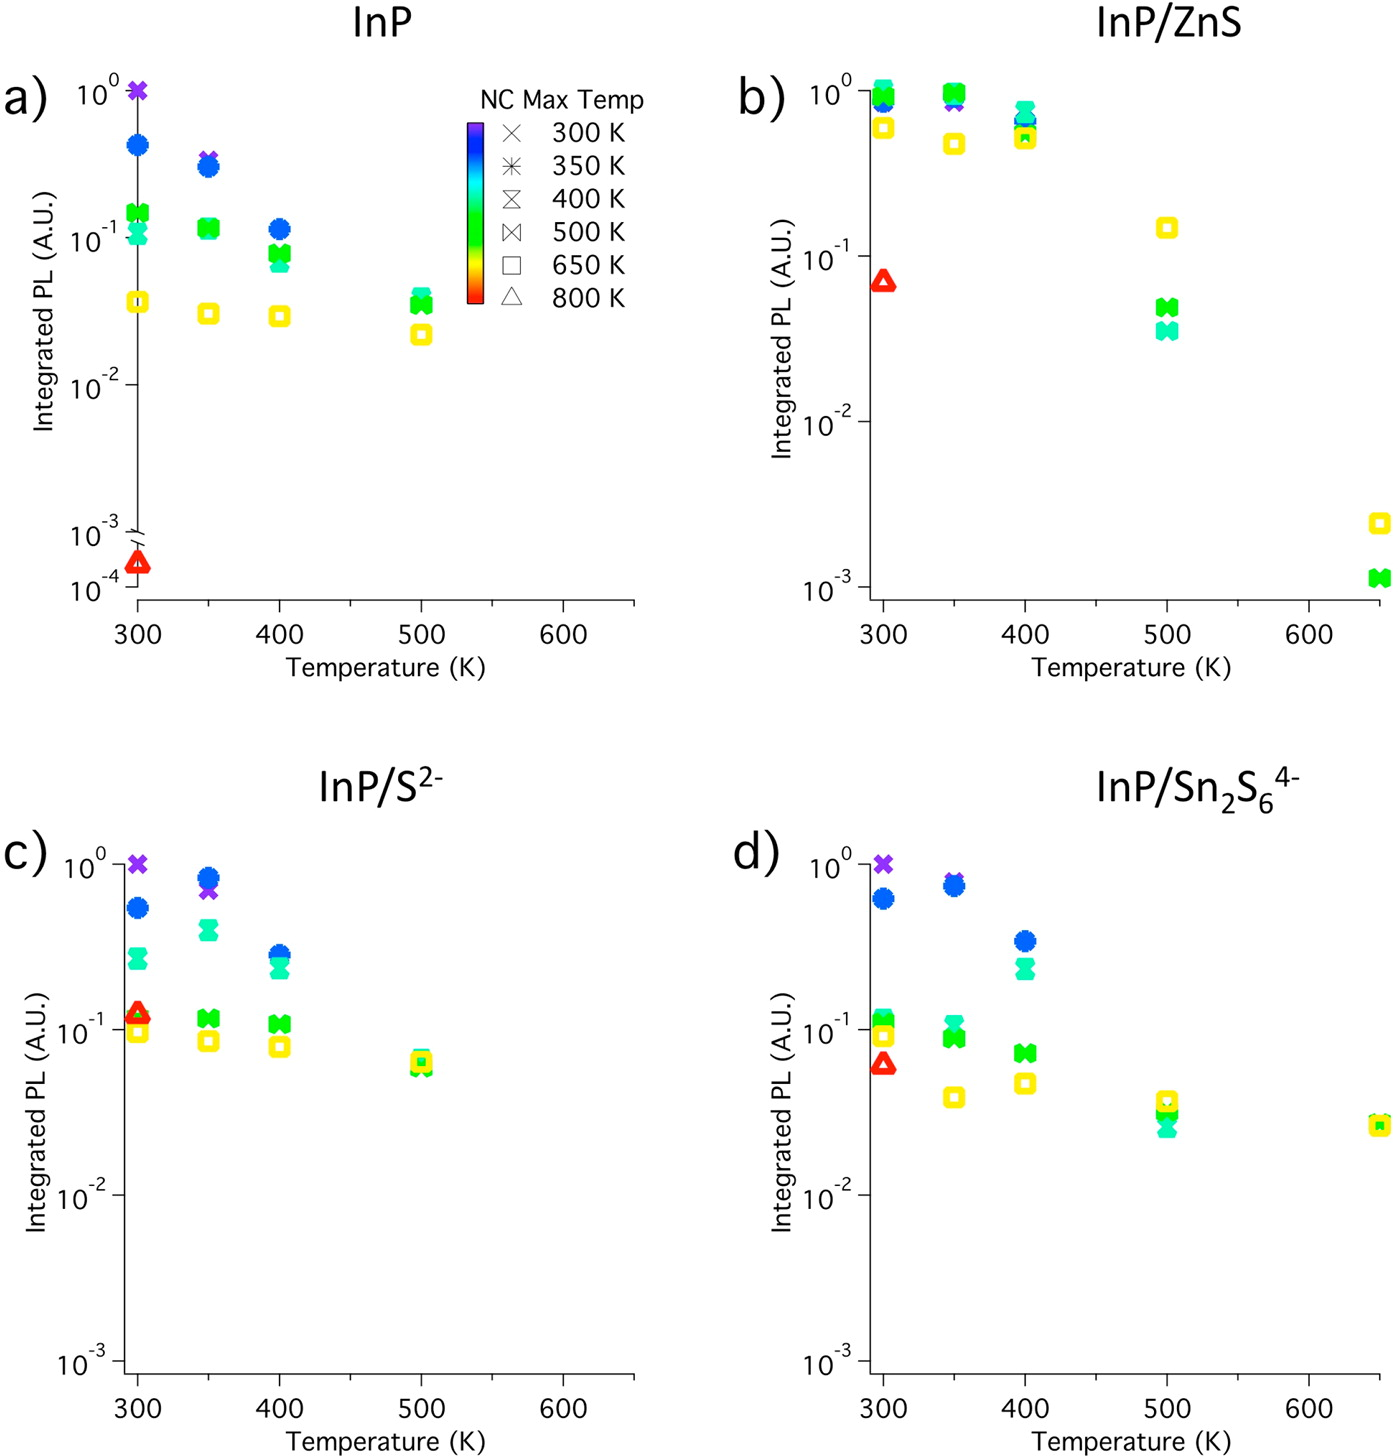
\includegraphics[width=\textwidth]{./Chapter5/inp1.jpeg}
\caption[Integrated PL intensity from InP NCs with four different surface terminations at a variety of temperatures.]{Integrated static PL for InP, InP/ZnS core-shell, InP/S$^{2-}$, and InP/Sn$_2$S$_6^{4-}$ NCs subjected to cyclical heating. Data are plotted as a function of measurement temperature, and symbols and colors correspond to the maximum temperature to which NCs were raised in the previous heating cycle. InP/ZnS and InP/S$^{2-}$ recover more resiliently after heating than do InP and InP/Sn$_2$S$_6^{4-}$ NCs. Data collected and analzyed by Clare Rowland, Northwestern University.}
\label{f:inp1}
\end{center}
\end{figure}

The data presented in Fig. \ref{f:inp1}(a) reveal an order of magnitude loss in PL at 300 K for organically-passivated InP cores following temperature elevation to a mere 400 K, while InP/ZnS cores recover virtually all PL intensity across the same regime. Following heating to higher temperatures (650 K), the organically-passivated InP cores exhibit a loss of 98\% PL intensity as compared to 40\% loss for InP/ZnS core-shell NCs. InP NCs passivated with small, inorganic ligands (S$^{2-}$ and Sn$_2$S$_6^{4-}$) display an intermediate extent of PL recovery following heating, and outperform the organically-passivated InP in this respect by a significant margin. In particular, inorganically-capped samples exhibit appreciable PL even following heating to 800 K, similar to the core-shell sample. \par

These above results are particularly encouraging in light of the fact that the small, inorganic capping ligands examined in this study have been found to enable extremely carrier mobilities in NC films exceeding even those exhibited by organically-passivated samples \cite{talapin2009prospects, lee2011band}. Several factors are important in understanding the improved thermal stability of S$^{2-}$ passivated NCs including the relative thermal stability of the passivating ligand as well as potential differences in electronic structure between organically and inorganically passivated NCs. Theoretical modeling was used to investigate the potential impact of inorganic passivation on NC electronic structure.

\subsubsection{Calculation Details}
Faceted zinc-blende InP nanocrystals with a 1.6 nm-diameter were constructed and passivated with hydrogen and sulfur atoms. Hydrogen passivation was accomplished by placing hydrogen atoms at tetrahedral positions for any In and P atoms having fewer than four bonds. Sulfur passivation was accomplished by placing sulfur atoms in positions corresponding to the lowest energy structure for a S-passivated InP surface. \cite{deng2010surface}. This structure consists of sulfur atoms on the InP surface as well as a layer of sulfur atoms beneath the top layer of In atoms on (001) faces. DFT calculations were carried out using the Vienna Ab-Initio Simulation Package \cite{PhysRevB.54.11169} with the supplied Projector Augemented Wave (PAW) potentials for core electrons \cite{kresse1999ultrasoft}. The NC was placed in the center of an otherwise empty 30 $\times$ 30 $\times$ 30 \r{A} unit cell, which was found to be sufficiently large to prevent spurious interactions between periodic images of the NCs. Electronic structure calculations were carried out at the $\Gamma$ point in the Brillouin zone. Atomic positions for each structure were relaxed until the forces acting on each atom were less than 0.02 eV/\r{A}, after which the electronic density of states (DOS) was calculated for each particle.

\subsubsection{Results and Discussion}

\begin{figure}
\begin{center}
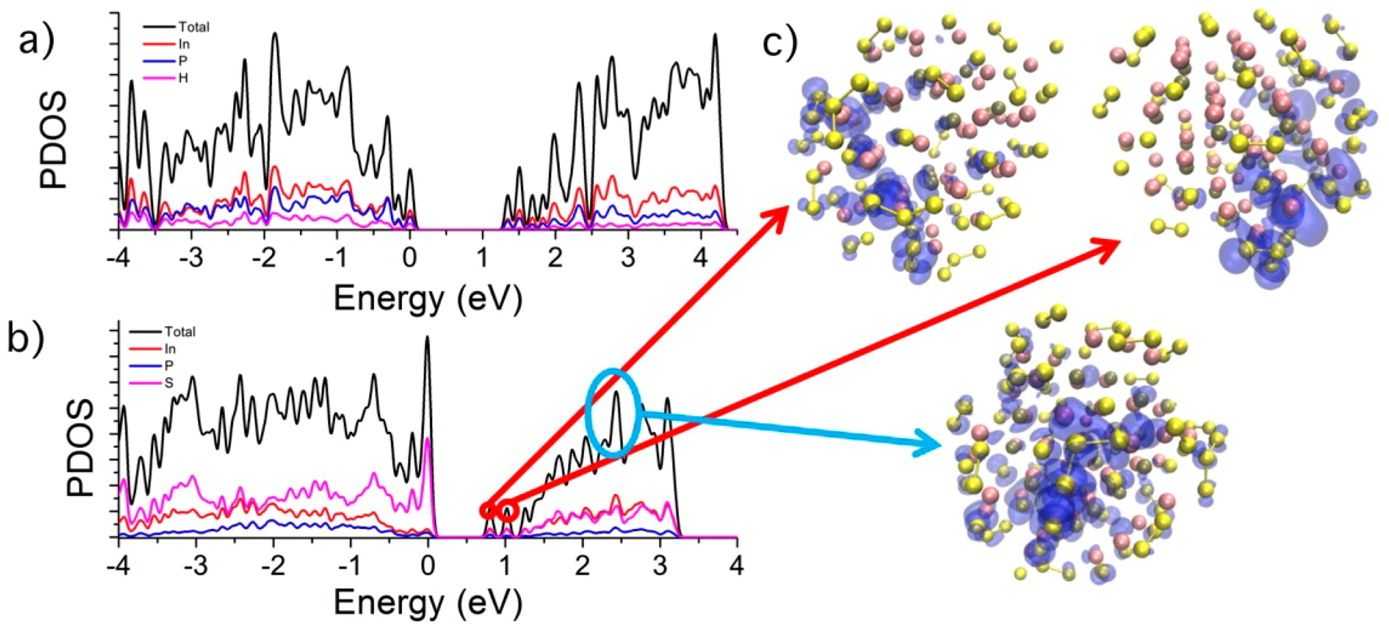
\includegraphics[width=\textwidth]{./Chapter5/inp2.jpeg}
\caption[DFT-dervied electronic structure of H- and S-passivated InP NCs.]{(a) DFT-derived electronic density of states for a hydrogen terminated InP nanocrystal (black curve). The PDOS for each atomic species is also shown: In (red curve), P (blue curve), H(pink curve). (b) DFT-derived electronic density of states for a sulfur terminated InP nanocrystal (black curve). The PDOS for each atomic species is also shown: In (red curve), P (blue curve), S(pink curve). (c) Lowest energy structure for a sulfur-terminated InP nanocrystal with three different charge densities, each associated with a region of the DOS indicated in (b). The red arrows indicate the trap-like states at the conduction band edge, while the blue arrow indicates a "core-like" state with charge density through the nanocrystal structure.}
\label{f:inp2}
\end{center}
\end{figure}

Figure \ref{f:inp2}(a) shows the total and atom-projected DOS for a hydrogen-terminated InP nanocrystal. The total DOS for the sulfur-terminated particle is shown in Figure \ref{f:inp2}(b). In each calculation, the highest occupied molecular orbital (HOMO) has been set to zero energy. Overall, the DOS is qualitatively similar for each structure, with a few exceptions. The valence band maximum for the sulfur terminated particle is dominated by contributions from sulfur atoms, in agreement with previous studies on sulfur-passivated InP (001) surfaces \cite{deng2010surface}. This contribution may be exaggerated compared to the nanocrystals studied experimentally, which are larger and have a correspondingly decreased surface-to-volume ratio. Two small bands are present at the bottom of the conduction band for the S-passivated nanocrystal (Figure \ref{f:inp2}(b)). We find these bands to have trap-like character, rather than being strongly associated with the NC core. Figure \ref{f:inp2}(c) shows the charge density associated with these states projected onto the NC structure. Circles and arrows drawn from Figure \ref{f:inp2}(b) indicate the origin of each charge density plot in Figure \ref{f:inp2}(c). The two small bands that are clearly below the main conduction band localize charge primarily in sulfur p-type orbitals and on In-S species on the NC surface. By contrast, states wholly within the conduction band exhibit charge density more evenly distributed through the NC, as shown in the bottom structure of Figure \ref{f:inp2}(c). Discounting the trap-like states at the conduction band minimum, we find similar energy gaps for the hydrogen-passivated and sulfur-passivated nanocrystal (1.35 and 1.37 eV, respectively). \par

\subsection{Conclusions}
These results suggest that the thermal stability imparted by passivation with inorganic ligands is not due to modification of the NC electronic structure. Instead, negligible differences in the electronic structure point to a temperature-driven change in atomistic conditions, the consideration of which merits a closer investigation of the thermal stability of the surface-passivating media. Degradation of the surface passivants would be expected to lead to surface defects and reconstructions, which would provide precisely the carrier trap sites that could account for irreversible PL loss. As is detailed in the work by Rowland \emph{et al.}, we ultimately attribute the superior high-T optical properties of S$^{2-}$-passivated InP to the extremely low volatility of the passivating ligand, which prevents temperature-induced desorption while still effectively passivating the NC surface. It is significant that S$^{2-}$ ligands do not perturb the NC electronic structure, as these ligands may provide a viable alternative to wide-gap shell growth which provides similar optical and thermal benefits whilst permitting electrical contact with the NC core. 

\subsection{The Impact of Covalent Surface Chemistry on the Thermal Stability of Si Nanocrystals}

\subsubsection{Background}
As demonstrated in this Chapter, the addition of a wide-gap semiconductor shell or small, inorganic passivating ligands such as $S^{2-}$ leads to improved optical performance of NC materials at elevated temperatures. However, most core-only NC compositions are passivated with ionically bound ligands, the volatility of which contributes to temperature-induced loss of desirable optical properties via the formation of trap sites at undercoordinated surface atoms \cite{rowland2013exciton, rowland2013thermal}. A key surface motif remaining unexplored is the covalent bond, the stability of which may yield more thermally robust surface passivation. \par

Silicon NCs are an excellent test bed for this motif given the ability of Si to form covalent bonds with carbon. Furthermore, Si dominates the electronics industry, and the enhanced optical properties of Si NCs relative to bulk Si has led to the suggestion that Si NCs may be useful in a wide variety of technologies. The optical properties of Si NCs are discussed at length the following Chapter. Excitement generated by the superior optical properties of Si NCs has been somewhat tempered by the apparently greatly depressed melting points of these materials, with prior reports noting melting in oxide-terminated Si NCs at as low as one-third of the bulk melting point \cite{goldstein1996melting, hirasawa2006size, lu2009size, wautelet1991estimation}. \par

To assess the role of covalent termination in NC stability, Si NPs terminated with covalently bound dodecane ligands were studied in a fashion similar to the InP NCs discussed in the previous section (see Fig. \ref{f:inp1}). The experimental details and results are reported in the work by Rowland \emph{et al.}\cite{rowland2014silicon}, but are summarized briefly here. \par

\subsubsection{Summary of Experimental Results}
Significant PL intensity was found to persist at temperatures up to 600 K, with PL losses up to 800 K being fully recoverable following a subsequent decrease in sample temperature. These results are surprising in light of previous reported experiments and theoretical work on melting point depression in Si NCs where particles in this size range (2-4 nm-diameter) have been reported to melt at 400 - 500 K \cite{goldstein1996melting, hirasawa2006size, lu2009size, wautelet1991estimation}. To support our experimental results, we analyzed covalently terminated Si NCs using an analytical model of nanocrystal melting as well as atomistic MD simulations. Both theoretical approaches are in agreement with our experimental results and suggest that surface passivation and lattice crystallinity persist well beyond 800 K for the sizes considered here. Overall these results suggest that covalent surface termination may offer optical and thermal benefits akin to shell growth. Our results also point to significantly higher melting points for covalently terminated NCs than those previously reported for oxide passivated particles.

\subsubsection{Phenomenological Model of Size-Dependent Nanocrystal Melting}
Theoretical descriptions of melting at surfaces and interfaces, and by logical extension, nanoparticles, constitute a field unto themselves, and a complete review of this subject is beyond of the scope of this thesis. Here, we focus on a thermodynamic, shape-sensitive model of nanocrystal melting that is well-suited to extremely small ($< \sim$2 nm) NCs \cite{farrell2007binding, wautelet2003phase}. While only some of the NCs experimentally considered fall in this regime, we are most interested in the lowest possible melting point expected for Si NCs considering prior reports of extremely low melting points relative to the bulk phase, and so choose to focus on a model which is known to accurately describe the melting points of the smallest sizes of NCs studied here. The model is derived from an expression of how the isobaric free energy of the (bulk) liquid phase, $G_l(T)$, varies with temperature as compared to the (bulk) crystalline phase, $G_c(T)$, for a fixed composition. Because the melting point, $T_m(\infty)$, is well above the Debye temperature of the solid, the specific heat is approximately constant. Then, the temperature variance of this Gibbs' free energy difference is given by Equation \ref{eq:simelting1}:
\begin{equation}\label{eq:simelting1}
(G_l - G_c)_{\infty} = C - BT
\end{equation}
In Eq. \ref{eq:simelting1}, $C/B = T_m(\infty)$, and $C$ is the latent heat of melting. In general, the $\infty$ subscript denotes the bulk phase. Computing a an analogous relationship for a finite-size cluster of $N$ atoms requires us to consider the effect of surface tensions for the solid and liquid phases:
\begin{equation}\label{eq:simelting2}
N(G_l - G_c) = N(G_l - G_c)_{\infty} + fN^{2/3}(\gamma_l - \gamma_c)
\end{equation}
In Eq. \ref{eq:simelting2}, $f$ is a geometrical factor depending on particle shape, and $\gamma_{l\left(c\right)}$ is the surface tension of the liquid (crystal). By definition, $(G_l - G_c) = 0$ at $T = T_m(r)$ for a particle of radius $r$. Therefore at $T = T_m(r)$, we have:
\begin{align*}
0 = N(G_l + G_c)_{\infty} + fN^{2/3}(\gamma_l - \gamma_c) 
\end{align*}
Plugging Eq. \ref{eq:simelting1} into the above and simplifying:
\begin{align*}
0 &= N(C - BT_m(r))_{\infty} + fN^{2/3}(\gamma_l - \gamma_c) \\
  &= C - BT_m(r) + fN^{-1/3}(\gamma_l - \gamma_c) \\
  &= \frac{C}{B} - T_m(r) + fN^{-1/3}\frac{(\gamma_l - \gamma_c)}{B}
\end{align*}
Recalling that $C/B = T_m(\infty)$, we substitute this into our equation and further simplify:
\begin{align*}
0 &= T_m(\infty) - T_m(r) + fN^{-1/3}\frac{(\gamma_l - \gamma_c)}{B}\\
T_m(r) &= T_m(\infty) + fN^{-1/3}\frac{(\gamma_l - \gamma_c)}{B} \\
T_m(r) &= T_m(\infty)\left[1 + fN^{-1/3}\frac{(\gamma_l - \gamma_c)}{BT_m(\infty)}\right] \\
\end{align*}
Finally, noting again that $BT_m(\infty) = C$, we arrive at Eq. \ref{eq:simelting3}:
\begin{equation}\label{eq:simelting3}
T_m(r) = T_m(\infty)\left[1 + fN^{-1/3}\frac{(\gamma_l - \gamma_c)}{C}\right] 
\end{equation}
The term $fN^{-1/3}$ is directly proportional to the ratio of surface to volume atoms \cite{wautelet2003phase}. Also, note that for a spherical particle, $N = r^3/(r_a^3)$, where $r_a$ is the atomic radius of the element in question. For a spherical particle, the $fN^{-1/3}$ may be recast purely in terms of the atomic radius:
\begin{align*} 
\frac{f}{N^{-1/3}} &= \frac{A}{V} \\
\frac{f}{r/r_a} &= \frac{4\pi r^2}{\left(4/3\right)\pi r^3} \\
\frac{f}{r/r_a} &= \frac{3}{r} \implies f = \frac{3}{r_a}
\end{align*}
Plugging this, along with the relationship between $N$ and $r_a$ described above, into Equation \ref{eq:simelting3} yields:
\begin{equation}\label{eq:simelting4}
T_m(r) = T_m(\infty) \left(1 - \frac{c'}{n}\right)
\end{equation}
In the above equation, $n = N^{1/3}$ and $c'$ is a collection of material-dependent constants: $c' = 3\left(\gamma_c - \gamma_l\right)/r_aC$. While addressing the specific case of small, group-IV semiconductor nanoparticles, Farrell and co-workers examined \emph{ab-initio} calculations of binding energy in these materials and $c'$ is roughly unity for small ($\sim$2 nm) particles and that the the linear dependence of $T_m(r)$ on $n$ is better described by a $1/n^2$ dependence than a $1/n$ dependence \cite{farrell2007binding}. Implementing these empirical corrections we arrive at the final expression for the dependence of nanoparticle melting point on cluster size:
\begin{equation}\label{eq:simelting5}
T_m(n) = T_m(\infty)\left[1 - \left(\frac{1}{n}\right)^2\right]
\end{equation}
While this model does predict NC $T_m$ size dependence, it does not account for atomistic details such as covalent surface chemistry, which may significantly impact thermal stability and $T_m$.

\subsubsection{Molecular Dynamics Simulations of Nanoparticle Melting}
We use MD simulations to gain atomistic insight into the temperature-dependent behavior of Si NCs. Faceted Si NCs were created using the Wulff construction and experimentally known surface energies \cite{hong1998effect}. For simplicity and computational tractability, Si NC surfaces were passivated with hydrogen atoms. Interactions between atoms were modeled using an empirical second-order reactive bond-order potential \cite{schall2008elastic}. The potential used here has been shown to reproduce well the elastic properties of crystalline Si and the energetics of the H-passivated Si surfaces \cite{murty1995empirical}. Si NCs were first relaxed until the forces between atoms were less than 0.02 eV/\r{A}. Following relaxation, NCs were subjected to a temperature annealing procedure. Atomic velocities were rescaled to a particular temperature in steps of 100 K. After each rescaling, NCs were allowed to equilibrate for 5 ps in the NVT ensemble. Following equilibration, NCs were simulated for another 2 ps to yield production-run data. All MD calculations were carried out using the General Utility Lattice Program \cite{gale2003general}. \par

\begin{figure}
\begin{center}
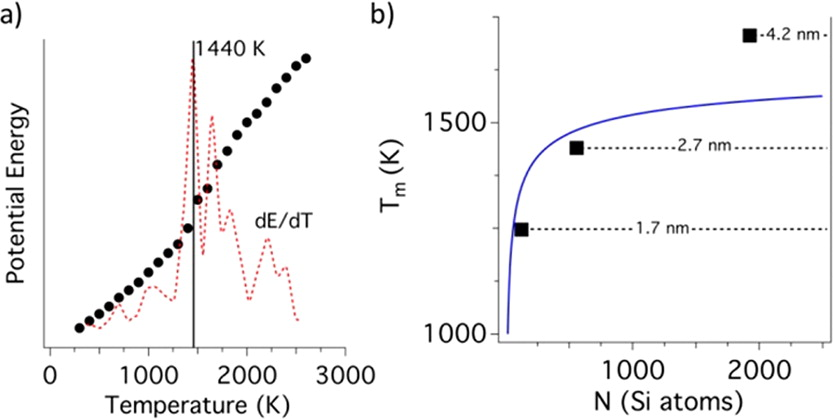
\includegraphics[width=\textwidth]{./Chapter5/simelting1.jpeg}
\caption[MD simulations of Si NC melting for multiple NC sizes.]{(a) Average potential energy vs temperature for a 2.6 nm-diameter, H-passivated Si NC. The data points represent an average of 2 ps of simulation of an equilibrated NC at the given temperature. The dashed line indicates the first derivative of the potential energy vs temperature. (b) Melting point as a function of Si NC temperature via multiple methods. The solid blue line indicates the prediction of the modified phenomenological model (Eq. \ref{eq:simelting5}), while the square data points indicate first derivative maxima indicating melting temperatures from MD simulations.}
\label{f:simelting1}
\end{center}
\end{figure}

Figure \ref{f:simelting1} displays the potential energy of a 2.6 nm Si NC (558 atoms) at each temperature step, averaged over the 2 ps production run. A discontinuity, emphasized in the first derivative, is evident at 1440 K and indicates a solid-liquid transition ($T_m$) that is depressed relative to $T_{m, bulk} = 1687$ K \cite{goldstein1992melting}. By similarly treating both a smaller and larger Si NC, a positive correlation appears between size and $T_m$, consistent with thermodynamic considerations. The MD simulations qualitatively agree with the phenomenonological model and prior MD studies utilizing the Stillinger-Weber potential \cite{fang2005investigation}. Agreement with the model is markedly poorer for the 4.2 nm particle, although this is perhaps not surprising in light of the fact that the model here was developed with extremely small particles in mind. Furthermore, the melting point of the largest particle seems to approach $T_{m, bulk}$; this is perhaps because the interaction potential utilized herein is known overestimate $T_{m, bulk}$ \cite{erhart2005analytical}. Regardless, both methods predict that $T_m$ values exceed the temperatures examined experimentally even for the smallest size of NC considered. \par
\subsection{Conclusions}
While the potential utilized in these MD simulations is parameterized to capture bond breaking and formation \cite{schall2008elastic}, the simulations do not exhibit ligand desorption until temperatures in excess of 1600 K. While further investigation is certainly warranted to model this process with a higher degree of accuracy, our theoretical effots support the conclusions suggested by the PL data presented in the work by Rowland \emph{et al.} \cite{rowland2014silicon}: Covalently-passivated Si NCs exhibit enhanced thermal stability relative to ionically-capped nanocrystals such as CdSe and InP.